\begin{activity}\label{A:0.5.1}
    In this activity we will review the trigonometry of the special angles $0^\circ$,
    $30^\circ$, $45^\circ$, and their multiples.
    \ba
        \item Use the fact that $180^\circ$ is the same as $\pi$ radians, convert each of
            the following angle measurements to radians.
            \begin{center}
                \begin{tabular}{|c||c|c|c|c|c|c|c|c|c|}
                    \hline
                    Degrees & $0^\circ$ & $30^\circ$ & $45^\circ$ & $60^\circ$ &
                    $90^\circ$ & $120^\circ$ & $135^\circ$ & $150^\circ$ & $180^\circ$ \\ \hline
                    Radians & 0 & & & & & & & & $\pi$ \\ \hline
                    \hline 
                    Degrees & $210^\circ$ & $225^\circ$ & $240^\circ$ & $270^\circ$ &
                    $300^\circ$ & $315^\circ$ & $330^\circ$ & $360^\circ$ &  \\ \hline
                    Radians & & & & & & & & & \\ \hline
                \end{tabular}
            \end{center}
        \item In part (a) of this problem there are several patterns that can help in
            remembering the radian conversions for certain angles.  For example, you
            should have found that $30^\circ$ converts to $\frac{\pi}{6}$ radians.
            Therefore, $60^\circ$ should be twice $\frac{\pi}{6}$ which indeed it is:
            $60^\circ = \frac{\pi}{3}$ radians.  What other similar patterns can you find?
            What is the minimum number of radian measures that you need to memorize?
        \item The sides of a $30-60-90$ triangle follow well-known ratios.  Consider the
            equilateral triangle on the left of the figure below.  Fill in the rest of the
            sides and angles on the figure and use them to determine the trigonometric values of $30^\circ$ and
            $60^\circ$.
            \begin{center}
                \begin{tabular}{|c|c||c|c|c|}
                    \hline
                    Angle (degrees) & Angle (radians) & Sine & Cosine & Tangent \\ \hline
                    \hline
                    $30^\circ$ & & & & \\ \hline
                    $60^\circ$ & & & & \\ \hline
                \end{tabular}
            \end{center}
        \item The sides of a $45-45-90$ triangle also follow well-known ratios.  Consider
            the isosceles triangle on the right of the figure below.  Fill in the rest of
            the sides and angles on the figure and use them to determine the trigonometric
            values of $45^\circ$.
            \begin{center}
                \begin{tabular}{|c|c||c|c|c|}
                    \hline
                    Angle (degrees) & Angle (radians) & Sine & Cosine & Tangent \\ \hline
                    \hline
                    $45^\circ$ & & & & \\ \hline
                \end{tabular}
            \end{center}
    \begin{center}
        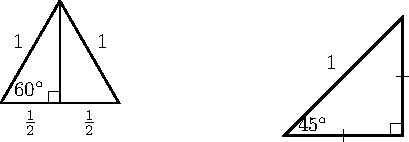
\includegraphics[width=0.5\columnwidth]{figures/0-5-fig_specialright.pdf}
    \end{center}
        \item Finally, we can organize all of the information about the special right
            triangles on a well-known organizational tool: the unit circle.  
    \begin{center}
        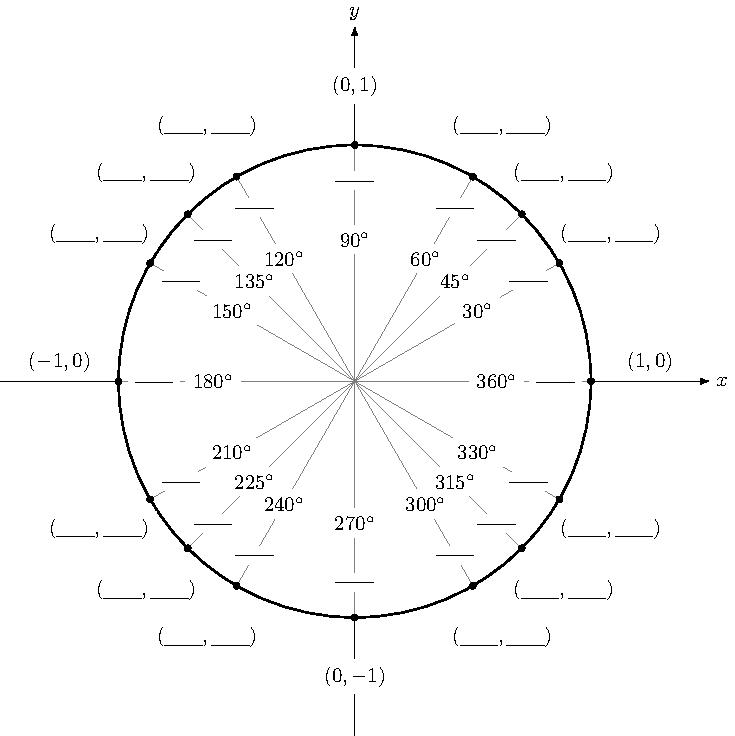
\includegraphics[width=0.7\columnwidth]{figures/0-5-UnitCircle.pdf}
    \end{center}
    \ea

\end{activity}
\begin{smallhint}
\end{smallhint}
\begin{bighint}
\end{bighint}
\begin{activitySolution}
    \begin{center}
        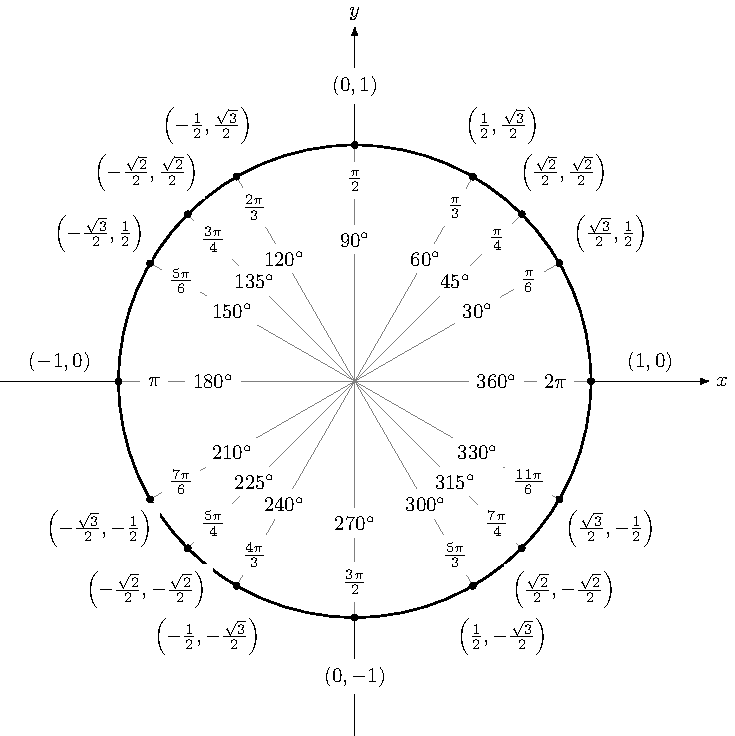
\includegraphics[width=0.6\columnwidth]{figures/0-5-UnitCircle_FilledIn.pdf}
    \end{center}
\end{activitySolution}

\aftera
